\section{实验结果与比较}

\subsection{严格课内主线}

严格课内版的结果先单独看。因为这是单标签四分类，exact-match 是更直接的指标，label-wise accuracy 只作为辅助参考。

这次严格课内版做了两处仍然属于课堂边界内的改动：一方面，不再只用四个 case 音频当模板，而是先把训练集同类样本的最大能量块平均成类别模板，再在选定块长后用 train+dev 重新估计最终模板；另一方面，在 dev 集上从 3--6 帧里选块长度，扩大数据集后最终选中 5 帧。数据词表从 60 个扩到 300 个以后，strict 版本面对的跨词变化更大，所以分数比小词表实验低，但它仍然保留了完整、可解释的课堂链路。

\begin{table}[H]
    \centering
    \caption{严格课内 FFT 模板法的主指标}
    \label{tab:strict-main}
    \begin{tabular}{lccccc}
        \toprule
        方法 & label-wise acc. & exact-match acc. & macro-F1 & micro-F1 & samples-F1 \\
        \midrule
        strict\_course\_fft & 0.6327 & 0.2655 & 0.2439 & 0.2655 & 0.2655 \\
        \bottomrule
    \end{tabular}
\end{table}

\begin{table}[H]
    \centering
    \caption{严格课内 FFT 模板法的分标签 F1}
    \label{tab:strict-per-label}
    \begin{tabular}{lcccc}
        \toprule
        方法 & /g/ & /b/ & /d/ & /z/ \\
        \midrule
        strict\_course\_fft & 0.217 & 0.163 & 0.243 & 0.353 \\
        \bottomrule
    \end{tabular}
\end{table}

图~\ref{fig:strict-score-dist} 进一步把四个标签的分数分布画出来。正样本和负样本有一定分离，但重叠仍然明显，所以严格课内版能说明任务，却还不够稳。

\begin{figure}[H]
    \centering
    \begin{minipage}{0.48\textwidth}
        \centering
        
\includegraphics[width=\linewidth]{figures/mswc_course_gbdz_75w_cap40_5_5/strict_course/score_distribution_g.png}
        \small /g/
    \end{minipage}\hfill
    \begin{minipage}{0.48\textwidth}
        \centering
        
\includegraphics[width=\linewidth]{figures/mswc_course_gbdz_75w_cap40_5_5/strict_course/score_distribution_b.png}
        \small /b/
    \end{minipage}

    \vspace{0.5em}
    \begin{minipage}{0.48\textwidth}
        \centering
        
\includegraphics[width=\linewidth]{figures/mswc_course_gbdz_75w_cap40_5_5/strict_course/score_distribution_d.png}
        \small /d/
    \end{minipage}\hfill
    \begin{minipage}{0.48\textwidth}
        \centering
        
\includegraphics[width=\linewidth]{figures/mswc_course_gbdz_75w_cap40_5_5/strict_course/score_distribution_z.png}
        \small /z/
    \end{minipage}
    \caption{严格课内版四个标签的得分分布。}
    \label{fig:strict-score-dist}
\end{figure}

\subsection{AI 重做版对照}

严格课内版之外，本文把 \texttt{course\_filterbank\_corr} 作为 AI 重做版的主要实现。它不是简单换一个分类器，而是重做前两步：先用 log-mel 与能量变化得到更稳的词首局部谱，再用正负模板差分和自相关完成检测。

\begin{table}[H]
    \centering
    \small
    \setlength{\tabcolsep}{4pt}
    \caption{严格课内版与 AI 重做版的整体比较}
    \label{tab:course-compare}
    \begin{tabular}{lccccc}
        \toprule
        方法 & label-wise acc. & exact-match acc. & macro-F1 & micro-F1 & samples-F1 \\
        \midrule
        strict\_course\_fft & 0.6327 & 0.2655 & 0.2439 & 0.2655 & 0.2655 \\
        course\_filterbank\_corr & 0.7513 & 0.5026 & 0.4974 & 0.5026 & 0.5026 \\
        \bottomrule
    \end{tabular}
\end{table}

\begin{table}[H]
    \centering
    \caption{严格课内版与 AI 重做版的分标签 F1}
    \label{tab:course-per-label}
    \begin{tabular}{lcccc}
        \toprule
        方法 & /g/ & /b/ & /d/ & /z/ \\
        \midrule
        strict\_course\_fft & 0.217 & 0.163 & 0.243 & 0.353 \\
        course\_filterbank\_corr & 0.464 & 0.359 & 0.429 & 0.737 \\
        \bottomrule
    \end{tabular}
\end{table}

AI 重做版的提升主要来自两点：它把搜索范围更精确地收到词首附近，也把局部窗里的正负模板差分显式算进去了。/z/ 的提升最大，说明持续摩擦音在 log-mel 局部模板和自相关线索里更稳定；/b/ 和 /d/ 的重叠仍然明显，短促爆破和对齐误差仍然会削弱模板证据。

\begin{figure}[H]
    \centering
    
\includegraphics[width=0.95\textwidth]{figures/mswc_course_gbdz_75w_cap40_5_5/letter_examples.png}
    \caption{AI 重做版对应的四个代表样本。}
    \label{fig:ext-examples}
\end{figure}

\begin{figure}[H]
    \centering
    
\includegraphics[width=0.90\textwidth]{figures/mswc_course_gbdz_75w_cap40_5_5/template_grid.png}
    \caption{AI 重做版使用的平均 log-mel 模板视角。它展示的是每类训练样本的平均谱图，不等同于正负差分模板，但能帮助观察四类词首能量分布。}
    \label{fig:ext-template-grid}
\end{figure}

图~\ref{fig:course-score-dist} 把 AI 重做版四个标签的测试得分分布单独列出。相比严格课内版，/z/ 的正负样本分离最明显；/g/、/b/、/d/ 仍然有重叠，这解释了为什么 AI 重做版提升明显但没有完全解决爆破音之间的混淆。

\begin{figure}[H]
    \centering
    \begin{minipage}{0.48\textwidth}
        \centering
        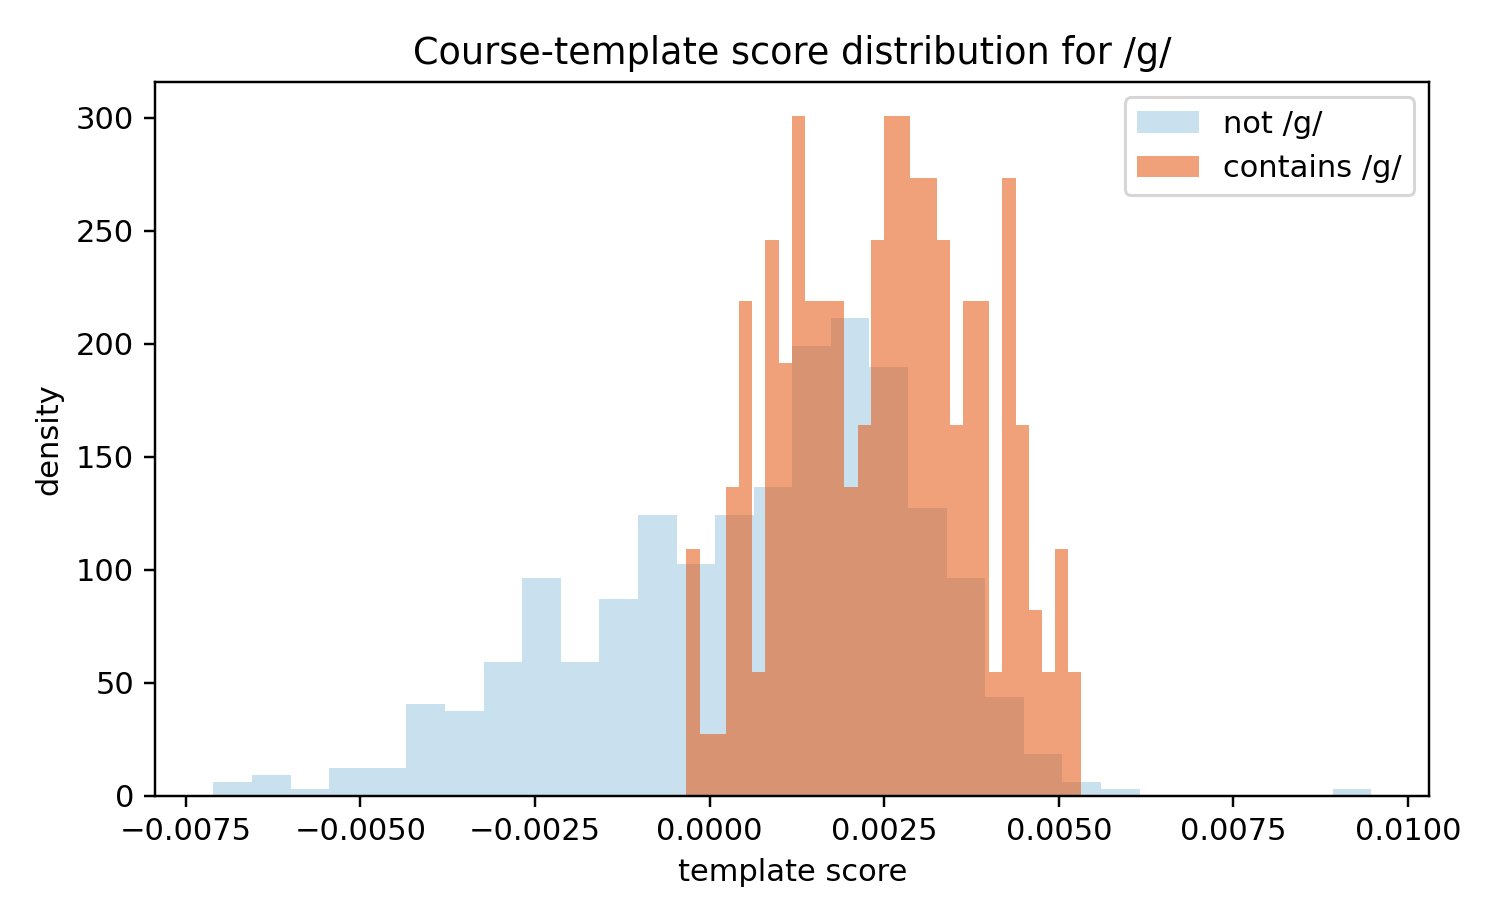
\includegraphics[width=\linewidth]{figures/mswc_course_gbdz_75w_cap40_5_5/course_filterbank_corr/score_distribution_g.png}
        \small /g/
    \end{minipage}\hfill
    \begin{minipage}{0.48\textwidth}
        \centering
        
\includegraphics[width=\linewidth]{figures/mswc_course_gbdz_75w_cap40_5_5/course_filterbank_corr/score_distribution_b.png}
        \small /b/
    \end{minipage}

    \vspace{0.5em}
    \begin{minipage}{0.48\textwidth}
        \centering
        
\includegraphics[width=\linewidth]{figures/mswc_course_gbdz_75w_cap40_5_5/course_filterbank_corr/score_distribution_d.png}
        \small /d/
    \end{minipage}\hfill
    \begin{minipage}{0.48\textwidth}
        \centering
        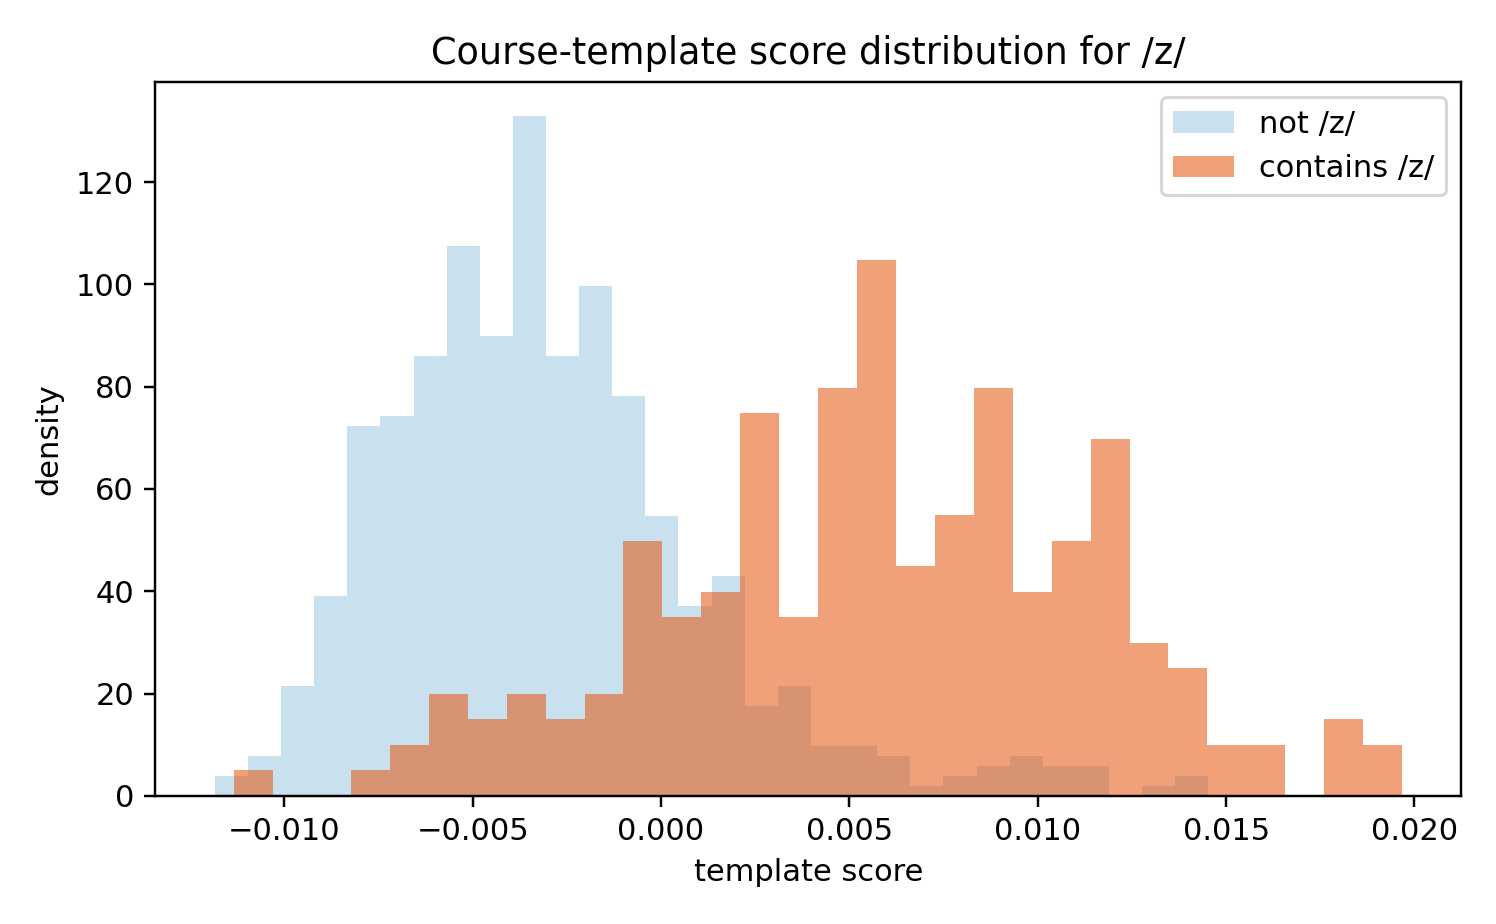
\includegraphics[width=\linewidth]{figures/mswc_course_gbdz_75w_cap40_5_5/course_filterbank_corr/score_distribution_z.png}
        \small /z/
    \end{minipage}
    \caption{\texttt{course\_filterbank\_corr} 四个标签的得分分布。}
    \label{fig:course-score-dist}
\end{figure}
